% Options for packages loaded elsewhere
\PassOptionsToPackage{unicode}{hyperref}
\PassOptionsToPackage{hyphens}{url}
%
\documentclass[
]{article}
\usepackage{amsmath,amssymb}
\usepackage{iftex}
\ifPDFTeX
  \usepackage[T1]{fontenc}
  \usepackage[utf8]{inputenc}
  \usepackage{textcomp} % provide euro and other symbols
\else % if luatex or xetex
  \usepackage{unicode-math} % this also loads fontspec
  \defaultfontfeatures{Scale=MatchLowercase}
  \defaultfontfeatures[\rmfamily]{Ligatures=TeX,Scale=1}
\fi
\usepackage{lmodern}
\ifPDFTeX\else
  % xetex/luatex font selection
\fi
% Use upquote if available, for straight quotes in verbatim environments
\IfFileExists{upquote.sty}{\usepackage{upquote}}{}
\IfFileExists{microtype.sty}{% use microtype if available
  \usepackage[]{microtype}
  \UseMicrotypeSet[protrusion]{basicmath} % disable protrusion for tt fonts
}{}
\makeatletter
\@ifundefined{KOMAClassName}{% if non-KOMA class
  \IfFileExists{parskip.sty}{%
    \usepackage{parskip}
  }{% else
    \setlength{\parindent}{0pt}
    \setlength{\parskip}{6pt plus 2pt minus 1pt}}
}{% if KOMA class
  \KOMAoptions{parskip=half}}
\makeatother
\usepackage{xcolor}
\usepackage[margin=1in]{geometry}
\usepackage{graphicx}
\makeatletter
\def\maxwidth{\ifdim\Gin@nat@width>\linewidth\linewidth\else\Gin@nat@width\fi}
\def\maxheight{\ifdim\Gin@nat@height>\textheight\textheight\else\Gin@nat@height\fi}
\makeatother
% Scale images if necessary, so that they will not overflow the page
% margins by default, and it is still possible to overwrite the defaults
% using explicit options in \includegraphics[width, height, ...]{}
\setkeys{Gin}{width=\maxwidth,height=\maxheight,keepaspectratio}
% Set default figure placement to htbp
\makeatletter
\def\fps@figure{htbp}
\makeatother
\setlength{\emergencystretch}{3em} % prevent overfull lines
\providecommand{\tightlist}{%
  \setlength{\itemsep}{0pt}\setlength{\parskip}{0pt}}
\setcounter{secnumdepth}{-\maxdimen} % remove section numbering
\ifLuaTeX
  \usepackage{selnolig}  % disable illegal ligatures
\fi
\IfFileExists{bookmark.sty}{\usepackage{bookmark}}{\usepackage{hyperref}}
\IfFileExists{xurl.sty}{\usepackage{xurl}}{} % add URL line breaks if available
\urlstyle{same}
\hypersetup{
  pdftitle={Analysis and Report},
  pdfauthor={R.Riddell},
  hidelinks,
  pdfcreator={LaTeX via pandoc}}

\title{Analysis and Report}
\author{R.Riddell}
\date{2023-10-09}

\begin{document}
\maketitle

{
\setcounter{tocdepth}{1}
\tableofcontents
}
ABS DATA
\url{https://www.abs.gov.au/methodologies/data-region-methodology/2011-22\#data-downloads}
Melbourne Housing
\url{https://www.kaggle.com/datasets/anthonypino/melbourne-housing-market}
postcode to LGA
\url{https://www.abs.gov.au/AUSSTATS/abs@.nsf/DetailsPage/1270.0.55.006July\%202011?OpenDocument}

\hypertarget{introduction}{%
\section{Introduction}\label{introduction}}

The housing market changes can have ripple effects though large sections
of the economy, the effects can be seen in areas like consumer spending
or have a direct impact on the construction industry. Being able to have
a broader understanding of the factors that affect housing prices can
better equip peoples ability to make decisions when entering or exiting
the market
{[}\url{https://www.rba.gov.au/speeches/2019/sp-gov-2019-03-06.html\#}:\textasciitilde:text=They\%20influence\%20consumer\%20spending\%2C\%20including,value\%20of\%20collateral\%20for\%20loans.{]}.
This report will examine house prices in relation to some broader
factors that surround the housing market between 2016 - 2018 and seek to
shed some light on the key drivers at that time.

\hypertarget{data}{%
\section{Data}\label{data}}

The data used is from publicly available data sets and can be found at
\href{https://www.abs.gov.au/methodologies/data-region-methodology/2011-22\#data-downloads}{ABS
DATA},
\href{https://www.kaggle.com/datasets/anthonypino/melbourne-housing-market}{Melbourne
Housing},
\href{https://www.abs.gov.au/AUSSTATS/abs@.nsf/DetailsPage/1270.0.55.006July\%202011?OpenDocument}{Postcode/
LGA data}. Datasets were aggreated to create a single data set that is
used for this exploration and analysis.

\hypertarget{na-treatment}{%
\subsection{NA Treatment}\label{na-treatment}}

After assessing all the columns that had more than 20\% null values the
decision was made to drop them. It didn't make any clear sense to add 0
into these columns, the values were then assessed against the whole data
set and against the other data points in their suburb. The range was
reasonably significant on both counts so mean imputation didn't seem
practical. The observations that included no final price were also
dropped, as we are investigating the factors associated with price I
didn't want to synthetically create target values. Seven additional
values were dropped as they had some NA values in the Postcode/ Property
Count This has left the data set with \texttt{length(dat)} observations
and \texttt{length(colnames(dat))} variables. The columns dropped were
\texttt{cols\_to\_drop}.

also dropping sellerG, Address and Postcode plus changing date to only
be year

\hypertarget{explatory-analysis}{%
\section{Explatory Analysis}\label{explatory-analysis}}

\hypertarget{distribution}{%
\subsection{Distribution}\label{distribution}}

The numeric values were analysed using histograms. All were relatively
normal, the average number of house transfers shows a reasonable normal
distribution with some areas having significantly more. The ratio of
cars under five years showing some right hand skewness implying some
areas have a significant proportion of cars less than five years old.
There is no obvious reason to drop any of these values based on their
distribution.

\begin{verbatim}
## Saving 6.5 x 4.5 in image
## Saving 6.5 x 4.5 in image
\end{verbatim}

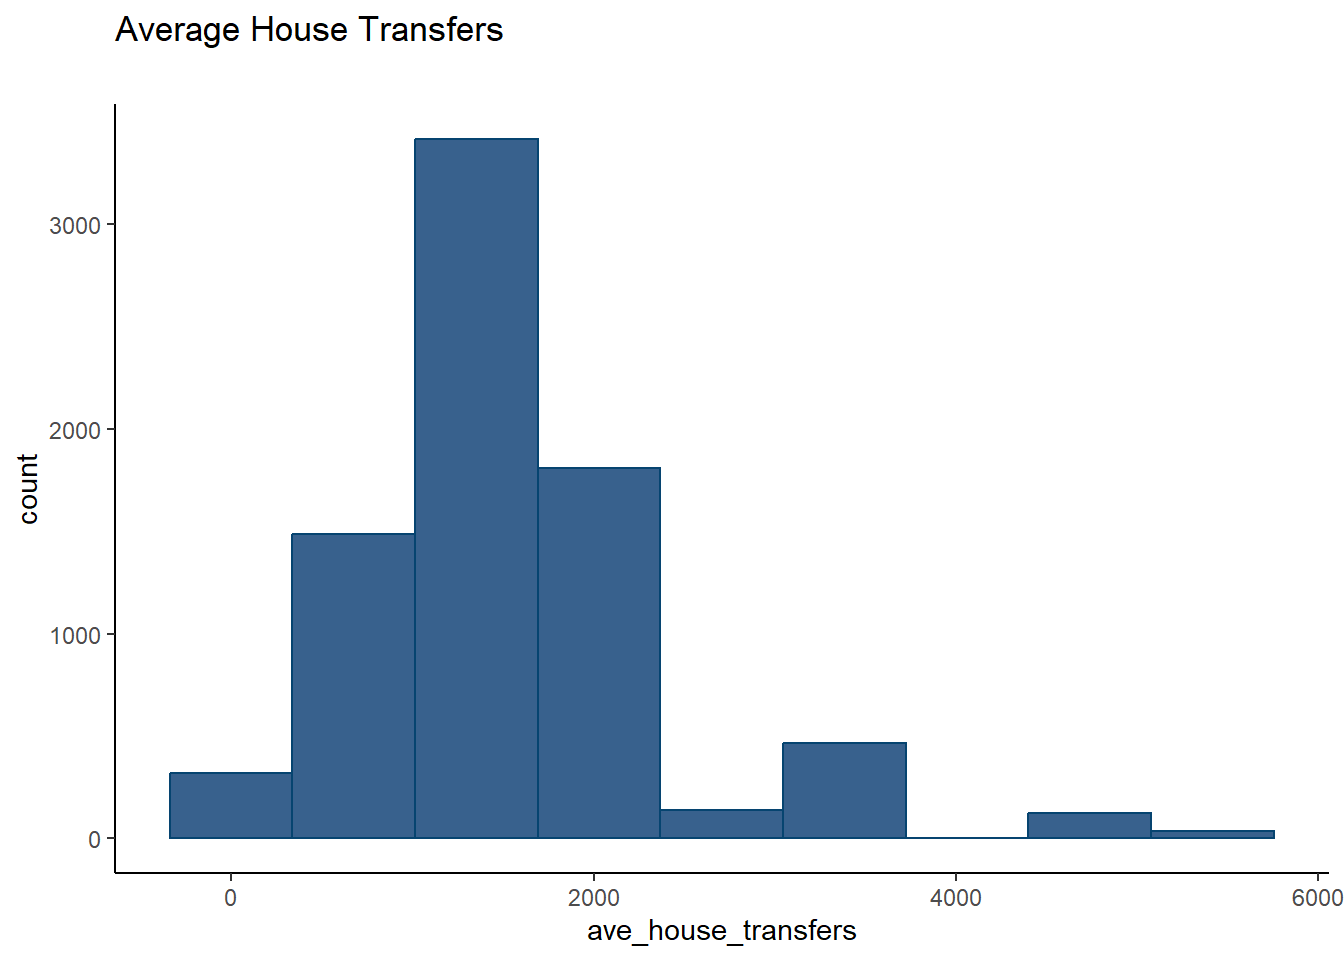
\includegraphics{Analysis-and-Report_files/figure-latex/histograms2-1.pdf}
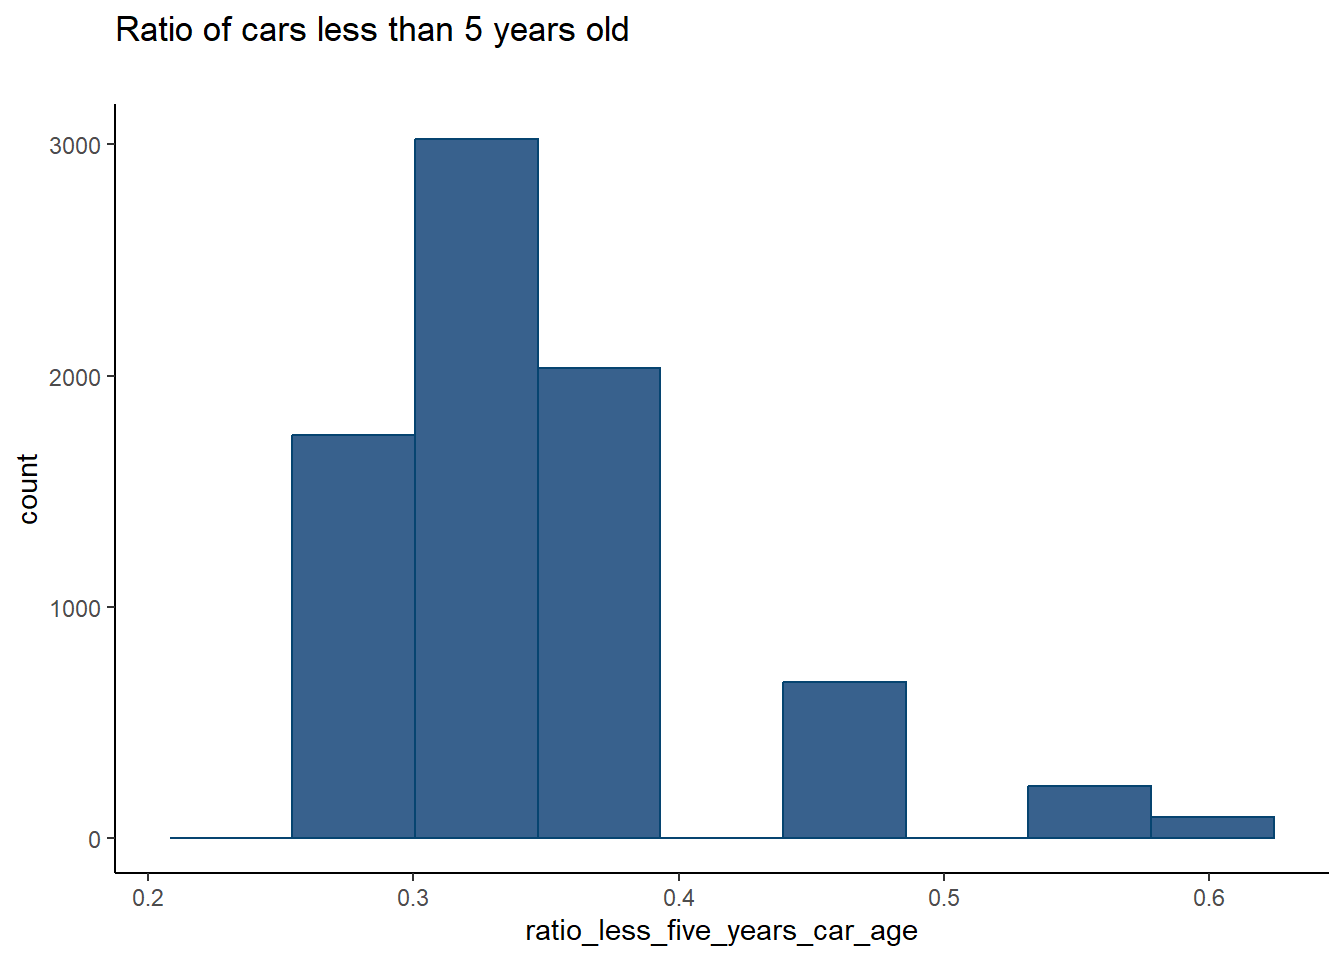
\includegraphics{Analysis-and-Report_files/figure-latex/histograms2-2.pdf}

The distribution of some of categorical variables was assessed against
the price. In some cases the distribution was significant across each
category and showed some potential outlines. In particular the most
common occupation shows that ``Professionals'' have significantly more
buying potential in some cases but their median is somewhat similar to
the other professions. When looking closer though the data set is
largely skewed by Professionals as they account for 86\% of the
responses. The Region Name also appears to be a factor in the price with
the regions who have the higher medians also have the biggest
distribution, this may point to the fact their is a house in every
region that is valued at the same price but it could be assumed not of
the same quality, size or age. Looking into the distribution of values
in the data set there does seem to be three regions providing rough 80\%
of the data, these areas are Southern Metropolitan, Northern
Metropolitan and Eastern. Metropolitan.

\begin{verbatim}
## Saving 6.5 x 4.5 in image
## Saving 6.5 x 4.5 in image
\end{verbatim}

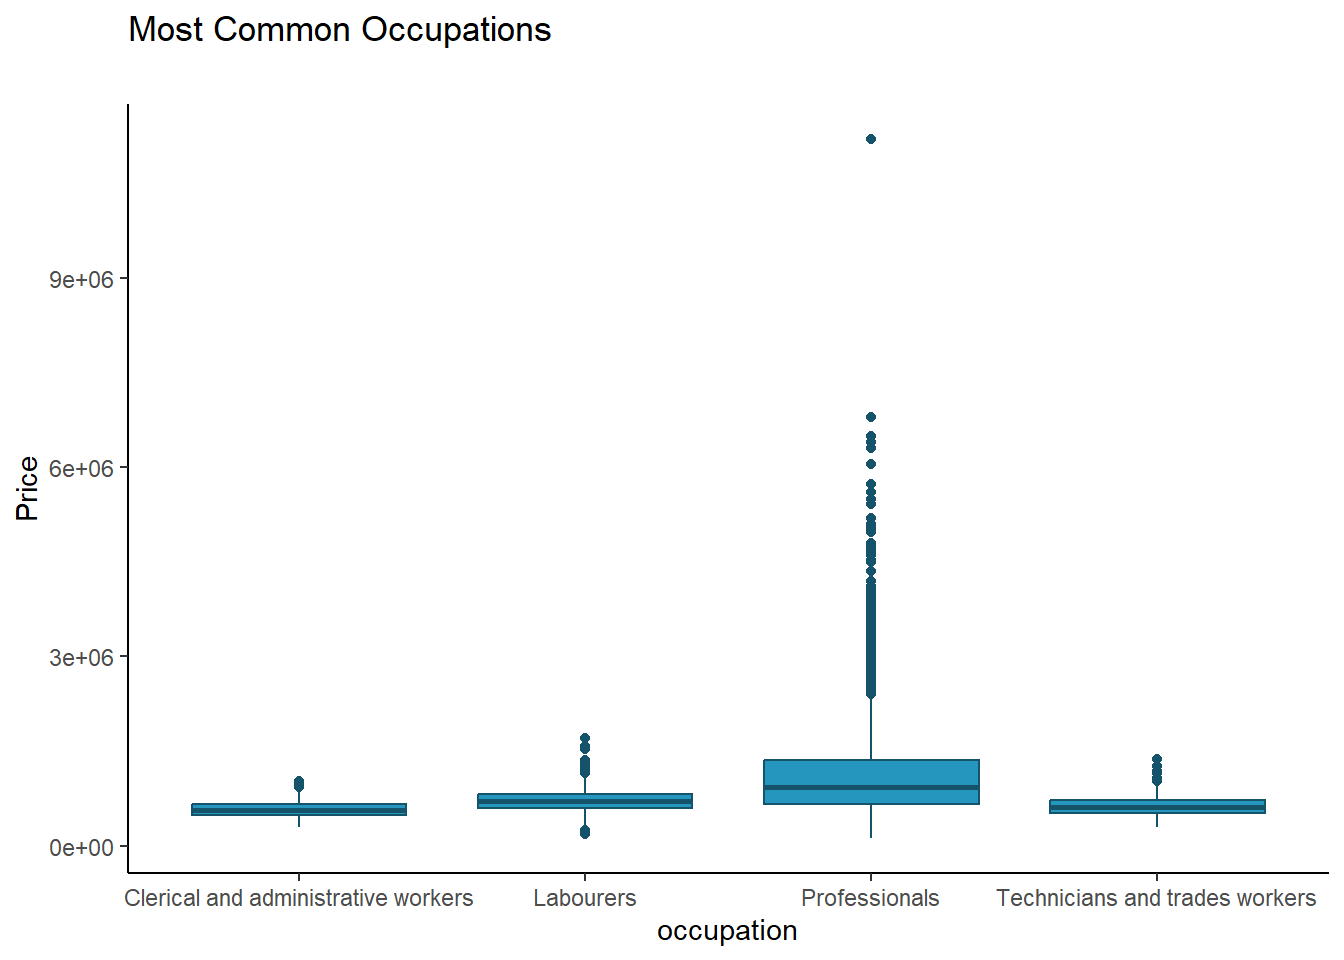
\includegraphics{Analysis-and-Report_files/figure-latex/box_plots2-1.pdf}
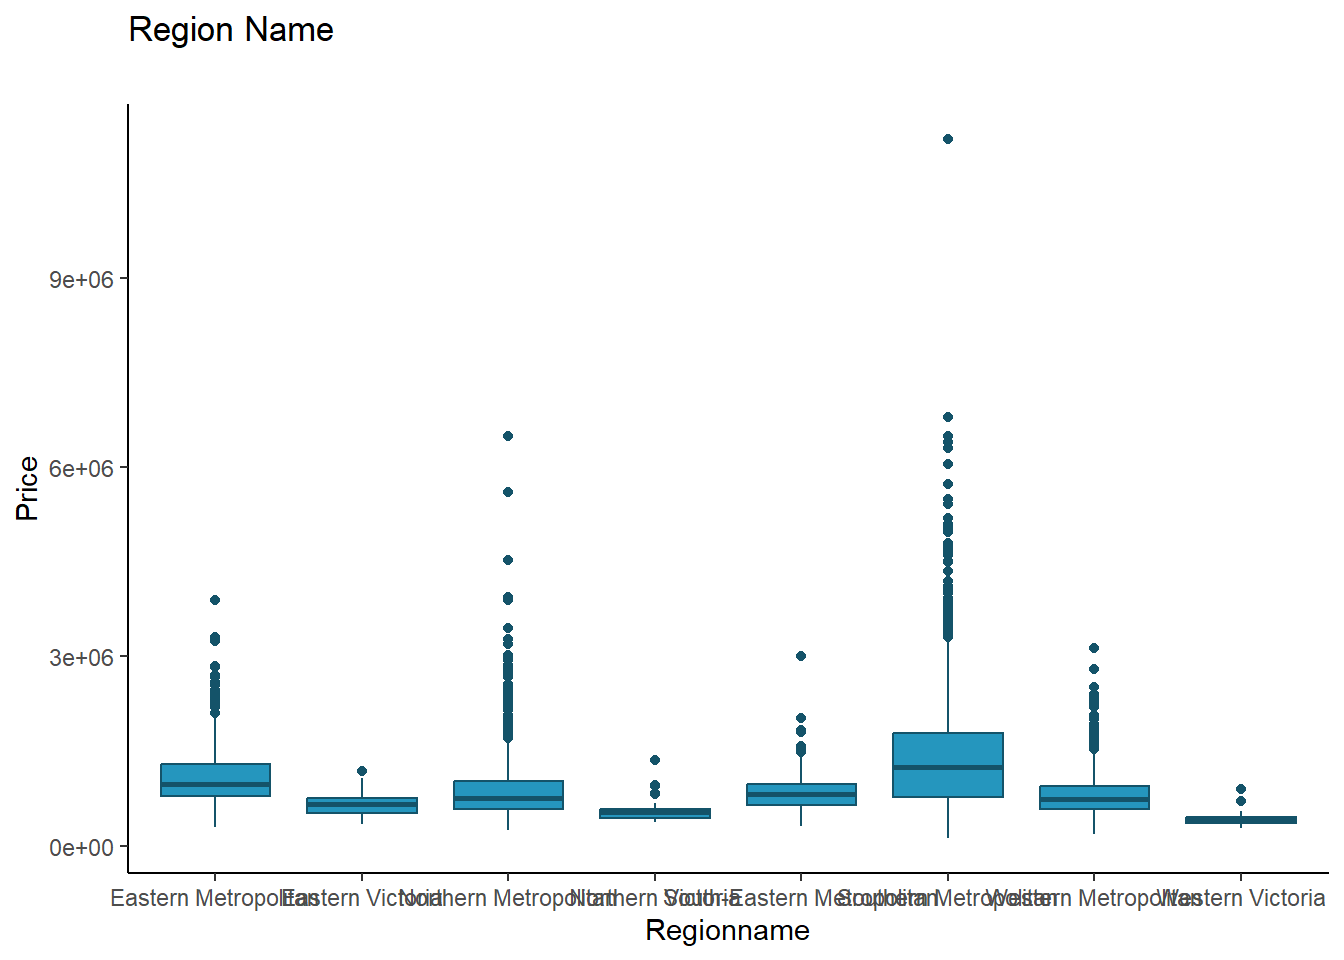
\includegraphics{Analysis-and-Report_files/figure-latex/box_plots2-2.pdf}

\hypertarget{relationships}{%
\subsection{Relationships}\label{relationships}}

The correlation coefficient of the numeric values against the price was
calculated. The Rooms variable showed the highest positive correlation
with a result of 0.44 showing that a property with more rooms may result
in a higher sale price. The strongest negative correlation was the
Distance from the CBD, this shows a slight relationship that when a
house is further from the CBD the sale price will be less. Purely from
the correlation coefficients the Property count and average total jobs
have been excluded as they are between -.10 and .10.

\hypertarget{assumption}{%
\section{Assumption}\label{assumption}}

Before attempting modelling it is important to check data to ensure it
fits the assumptions of the models. This process helps to select the
models that are most appropriate to the data, it will ensure a more
valid result and the model should be more reflective of the data and
therefore more accurate. As a starting point a linear model has been
created with the price as the target variable and it will be tested
against the assumption for the linear model.

\hypertarget{continous-variable}{%
\subsection{Continous Variable}\label{continous-variable}}

We are going to use a linear regression model so it is important that
the target variable is continuous.

\hypertarget{outliers}{%
\subsection{Outliers}\label{outliers}}

Using cooks distance and examining the residual plots we can see some
significant issues with how the data is represented by a linear model.
The Residual plot has an obvious pattern where is should be more random
With some. The Q-Q plot does not follow the line and has a significant
upwards curve.

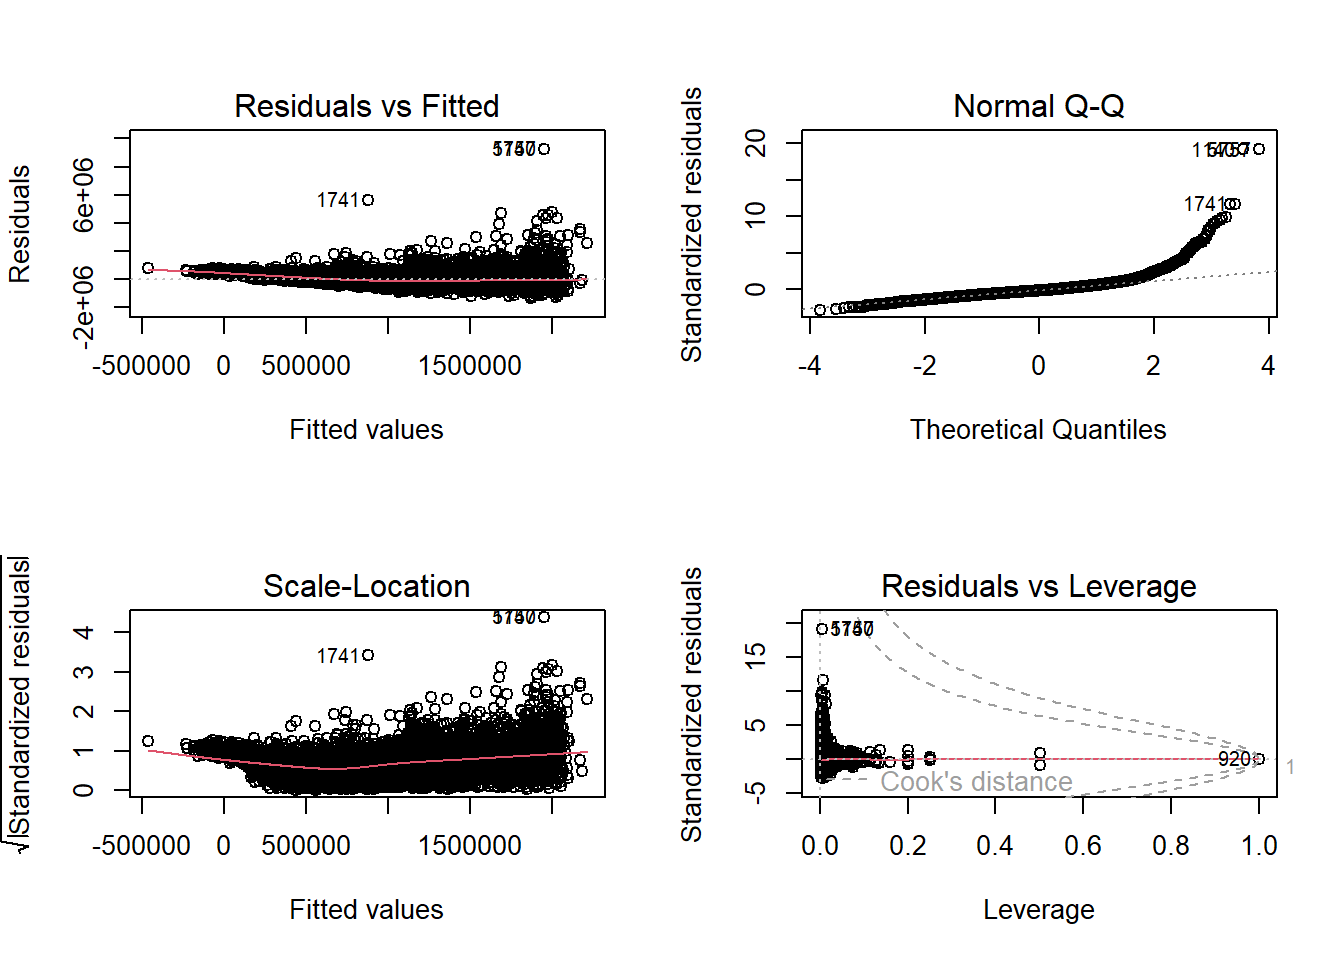
\includegraphics{Analysis-and-Report_files/figure-latex/residual plots-1.pdf}

As the residual plots showed the data was not well represented by linear
modelling it doesn't make sense to continue testing the linear modelling
assumptions against this data. Other tests that could be completed are
for homoscedasticity, near zero variance or multicolinearity. This
information has assisted in understanding what regression modelling
techniques may be suitable, as such the models chosen to test will be
random forest regression and KNN regression. KNN regression assumes that
the closer a data point is to another the more similar it will be.
Random forest regression (decision trees) assumes that data can be split
into subsets reasonable distinctly.

\hypertarget{modelling}{%
\section{Modelling}\label{modelling}}

The data is split randomly into two groups of testing and training, the
testing group is 20\% of the observations and the training is 80\%. The
training data is then used to build the models, once models are built
the testing data can be used to assess the RMSE and R squared. In the
model building phase there is also repeated cross validation. This
divides the data into into a number of partitions, with some partitions
not used for model building. The unused partitions can then be used as
an internal test and the mean performance is reported across the
iterations. Based on compute and time based factors the larger data set
has been re sampled down to 10,000 and the split 80/20 into training and
testing groups.

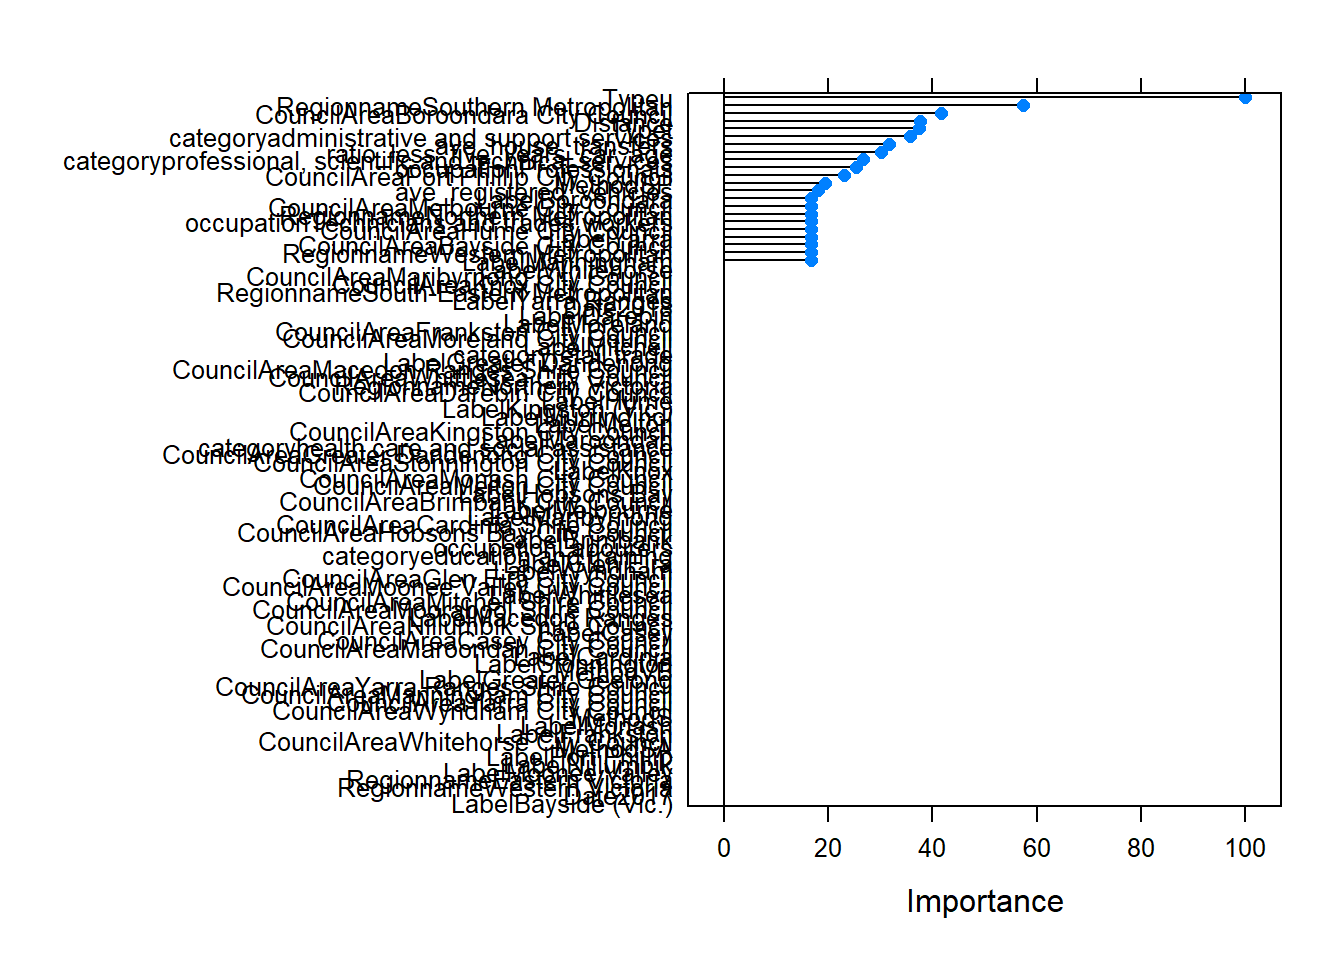
\includegraphics{Analysis-and-Report_files/figure-latex/rf model-1.pdf}

\begin{verbatim}
## rf variable importance
## 
##   only 20 most important variables shown (out of 92)
## 
##                                                         Overall
## Typeu                                                    100.00
## ratio_less_five_years_car_age                             85.44
## RegionnameSouthern Metropolitan                           62.87
## ave_house_transfers                                       57.34
## Distance                                                  49.12
## categoryprofessional, scientific and technical services   35.96
## LabelGlen Eira                                            32.96
## occupationProfessionals                                   32.59
## ave_registered_vehicles                                   32.30
## categoryadministrative and support services               32.25
## LabelBoroondara                                           27.14
## CouncilAreaManningham City Council                        22.75
## LabelWhittlesea                                           22.75
## LabelBayside (Vic.)                                       22.75
## CouncilAreaCasey City Council                             22.75
## LabelKnox                                                 22.75
## CouncilAreaHume City Council                              22.75
## CouncilAreaKingston City Council                          22.75
## CouncilAreaGlen Eira City Council                         22.75
## LabelMaribyrnong                                          22.75
\end{verbatim}

\begin{verbatim}
## Warning in preProcess.default(thresh = 0.95, k = 5, freqCut = 19, uniqueCut =
## 10, : These variables have zero variances: CouncilAreaMitchell Shire Council,
## LabelGreater Geelong, LabelMoorabool

## Warning in preProcess.default(thresh = 0.95, k = 5, freqCut = 19, uniqueCut =
## 10, : These variables have zero variances: CouncilAreaMitchell Shire Council,
## LabelGreater Geelong, LabelMoorabool

## Warning in preProcess.default(thresh = 0.95, k = 5, freqCut = 19, uniqueCut =
## 10, : These variables have zero variances: CouncilAreaMitchell Shire Council,
## LabelGreater Geelong, LabelMoorabool

## Warning in preProcess.default(thresh = 0.95, k = 5, freqCut = 19, uniqueCut =
## 10, : These variables have zero variances: CouncilAreaMitchell Shire Council,
## LabelGreater Geelong, LabelMoorabool

## Warning in preProcess.default(thresh = 0.95, k = 5, freqCut = 19, uniqueCut =
## 10, : These variables have zero variances: CouncilAreaMitchell Shire Council,
## LabelGreater Geelong, LabelMoorabool
\end{verbatim}

\begin{verbatim}
## Warning in preProcess.default(thresh = 0.95, k = 5, freqCut = 19, uniqueCut =
## 10, : These variables have zero variances: LabelMoorabool, LabelMurrindindi

## Warning in preProcess.default(thresh = 0.95, k = 5, freqCut = 19, uniqueCut =
## 10, : These variables have zero variances: LabelMoorabool, LabelMurrindindi

## Warning in preProcess.default(thresh = 0.95, k = 5, freqCut = 19, uniqueCut =
## 10, : These variables have zero variances: LabelMoorabool, LabelMurrindindi

## Warning in preProcess.default(thresh = 0.95, k = 5, freqCut = 19, uniqueCut =
## 10, : These variables have zero variances: LabelMoorabool, LabelMurrindindi

## Warning in preProcess.default(thresh = 0.95, k = 5, freqCut = 19, uniqueCut =
## 10, : These variables have zero variances: LabelMoorabool, LabelMurrindindi
\end{verbatim}

\begin{verbatim}
## Warning in preProcess.default(thresh = 0.95, k = 5, freqCut = 19, uniqueCut =
## 10, : These variables have zero variances: CouncilAreaMitchell Shire Council,
## LabelMoorabool

## Warning in preProcess.default(thresh = 0.95, k = 5, freqCut = 19, uniqueCut =
## 10, : These variables have zero variances: CouncilAreaMitchell Shire Council,
## LabelMoorabool

## Warning in preProcess.default(thresh = 0.95, k = 5, freqCut = 19, uniqueCut =
## 10, : These variables have zero variances: CouncilAreaMitchell Shire Council,
## LabelMoorabool

## Warning in preProcess.default(thresh = 0.95, k = 5, freqCut = 19, uniqueCut =
## 10, : These variables have zero variances: CouncilAreaMitchell Shire Council,
## LabelMoorabool

## Warning in preProcess.default(thresh = 0.95, k = 5, freqCut = 19, uniqueCut =
## 10, : These variables have zero variances: CouncilAreaMitchell Shire Council,
## LabelMoorabool
\end{verbatim}

\begin{verbatim}
## Warning in preProcess.default(thresh = 0.95, k = 5, freqCut = 19, uniqueCut =
## 10, : These variables have zero variances: LabelMurrindindi

## Warning in preProcess.default(thresh = 0.95, k = 5, freqCut = 19, uniqueCut =
## 10, : These variables have zero variances: LabelMurrindindi

## Warning in preProcess.default(thresh = 0.95, k = 5, freqCut = 19, uniqueCut =
## 10, : These variables have zero variances: LabelMurrindindi

## Warning in preProcess.default(thresh = 0.95, k = 5, freqCut = 19, uniqueCut =
## 10, : These variables have zero variances: LabelMurrindindi

## Warning in preProcess.default(thresh = 0.95, k = 5, freqCut = 19, uniqueCut =
## 10, : These variables have zero variances: LabelMurrindindi
\end{verbatim}

\begin{verbatim}
## Warning in preProcess.default(thresh = 0.95, k = 5, freqCut = 19, uniqueCut =
## 10, : These variables have zero variances: LabelMoorabool

## Warning in preProcess.default(thresh = 0.95, k = 5, freqCut = 19, uniqueCut =
## 10, : These variables have zero variances: LabelMoorabool

## Warning in preProcess.default(thresh = 0.95, k = 5, freqCut = 19, uniqueCut =
## 10, : These variables have zero variances: LabelMoorabool

## Warning in preProcess.default(thresh = 0.95, k = 5, freqCut = 19, uniqueCut =
## 10, : These variables have zero variances: LabelMoorabool

## Warning in preProcess.default(thresh = 0.95, k = 5, freqCut = 19, uniqueCut =
## 10, : These variables have zero variances: LabelMoorabool
\end{verbatim}

\begin{verbatim}
## Warning in preProcess.default(thresh = 0.95, k = 5, freqCut = 19, uniqueCut =
## 10, : These variables have zero variances: LabelMurrindindi

## Warning in preProcess.default(thresh = 0.95, k = 5, freqCut = 19, uniqueCut =
## 10, : These variables have zero variances: LabelMurrindindi

## Warning in preProcess.default(thresh = 0.95, k = 5, freqCut = 19, uniqueCut =
## 10, : These variables have zero variances: LabelMurrindindi

## Warning in preProcess.default(thresh = 0.95, k = 5, freqCut = 19, uniqueCut =
## 10, : These variables have zero variances: LabelMurrindindi

## Warning in preProcess.default(thresh = 0.95, k = 5, freqCut = 19, uniqueCut =
## 10, : These variables have zero variances: LabelMurrindindi
\end{verbatim}

\begin{verbatim}
## Warning in preProcess.default(thresh = 0.95, k = 5, freqCut = 19, uniqueCut =
## 10, : These variables have zero variances: LabelGreater Geelong, LabelMoorabool

## Warning in preProcess.default(thresh = 0.95, k = 5, freqCut = 19, uniqueCut =
## 10, : These variables have zero variances: LabelGreater Geelong, LabelMoorabool

## Warning in preProcess.default(thresh = 0.95, k = 5, freqCut = 19, uniqueCut =
## 10, : These variables have zero variances: LabelGreater Geelong, LabelMoorabool

## Warning in preProcess.default(thresh = 0.95, k = 5, freqCut = 19, uniqueCut =
## 10, : These variables have zero variances: LabelGreater Geelong, LabelMoorabool

## Warning in preProcess.default(thresh = 0.95, k = 5, freqCut = 19, uniqueCut =
## 10, : These variables have zero variances: LabelGreater Geelong, LabelMoorabool
\end{verbatim}

\begin{verbatim}
## Warning in preProcess.default(thresh = 0.95, k = 5, freqCut = 19, uniqueCut =
## 10, : These variables have zero variances: LabelMoorabool

## Warning in preProcess.default(thresh = 0.95, k = 5, freqCut = 19, uniqueCut =
## 10, : These variables have zero variances: LabelMoorabool

## Warning in preProcess.default(thresh = 0.95, k = 5, freqCut = 19, uniqueCut =
## 10, : These variables have zero variances: LabelMoorabool

## Warning in preProcess.default(thresh = 0.95, k = 5, freqCut = 19, uniqueCut =
## 10, : These variables have zero variances: LabelMoorabool

## Warning in preProcess.default(thresh = 0.95, k = 5, freqCut = 19, uniqueCut =
## 10, : These variables have zero variances: LabelMoorabool
\end{verbatim}

\begin{verbatim}
## Warning in preProcess.default(thresh = 0.95, k = 5, freqCut = 19, uniqueCut =
## 10, : These variables have zero variances: LabelMurrindindi

## Warning in preProcess.default(thresh = 0.95, k = 5, freqCut = 19, uniqueCut =
## 10, : These variables have zero variances: LabelMurrindindi

## Warning in preProcess.default(thresh = 0.95, k = 5, freqCut = 19, uniqueCut =
## 10, : These variables have zero variances: LabelMurrindindi

## Warning in preProcess.default(thresh = 0.95, k = 5, freqCut = 19, uniqueCut =
## 10, : These variables have zero variances: LabelMurrindindi

## Warning in preProcess.default(thresh = 0.95, k = 5, freqCut = 19, uniqueCut =
## 10, : These variables have zero variances: LabelMurrindindi
\end{verbatim}

\begin{verbatim}
## Warning in preProcess.default(thresh = 0.95, k = 5, freqCut = 19, uniqueCut =
## 10, : These variables have zero variances: LabelMoorabool, LabelMurrindindi

## Warning in preProcess.default(thresh = 0.95, k = 5, freqCut = 19, uniqueCut =
## 10, : These variables have zero variances: LabelMoorabool, LabelMurrindindi

## Warning in preProcess.default(thresh = 0.95, k = 5, freqCut = 19, uniqueCut =
## 10, : These variables have zero variances: LabelMoorabool, LabelMurrindindi

## Warning in preProcess.default(thresh = 0.95, k = 5, freqCut = 19, uniqueCut =
## 10, : These variables have zero variances: LabelMoorabool, LabelMurrindindi

## Warning in preProcess.default(thresh = 0.95, k = 5, freqCut = 19, uniqueCut =
## 10, : These variables have zero variances: LabelMoorabool, LabelMurrindindi
\end{verbatim}

\begin{verbatim}
## Warning in preProcess.default(thresh = 0.95, k = 5, freqCut = 19, uniqueCut =
## 10, : These variables have zero variances: LabelGreater Geelong,
## LabelMurrindindi

## Warning in preProcess.default(thresh = 0.95, k = 5, freqCut = 19, uniqueCut =
## 10, : These variables have zero variances: LabelGreater Geelong,
## LabelMurrindindi

## Warning in preProcess.default(thresh = 0.95, k = 5, freqCut = 19, uniqueCut =
## 10, : These variables have zero variances: LabelGreater Geelong,
## LabelMurrindindi

## Warning in preProcess.default(thresh = 0.95, k = 5, freqCut = 19, uniqueCut =
## 10, : These variables have zero variances: LabelGreater Geelong,
## LabelMurrindindi

## Warning in preProcess.default(thresh = 0.95, k = 5, freqCut = 19, uniqueCut =
## 10, : These variables have zero variances: LabelGreater Geelong,
## LabelMurrindindi
\end{verbatim}

\begin{verbatim}
## Warning in preProcess.default(thresh = 0.95, k = 5, freqCut = 19, uniqueCut =
## 10, : These variables have zero variances: CouncilAreaMitchell Shire Council,
## LabelGreater Geelong

## Warning in preProcess.default(thresh = 0.95, k = 5, freqCut = 19, uniqueCut =
## 10, : These variables have zero variances: CouncilAreaMitchell Shire Council,
## LabelGreater Geelong

## Warning in preProcess.default(thresh = 0.95, k = 5, freqCut = 19, uniqueCut =
## 10, : These variables have zero variances: CouncilAreaMitchell Shire Council,
## LabelGreater Geelong

## Warning in preProcess.default(thresh = 0.95, k = 5, freqCut = 19, uniqueCut =
## 10, : These variables have zero variances: CouncilAreaMitchell Shire Council,
## LabelGreater Geelong

## Warning in preProcess.default(thresh = 0.95, k = 5, freqCut = 19, uniqueCut =
## 10, : These variables have zero variances: CouncilAreaMitchell Shire Council,
## LabelGreater Geelong
\end{verbatim}

\begin{verbatim}
## Warning in preProcess.default(thresh = 0.95, k = 5, freqCut = 19, uniqueCut =
## 10, : These variables have zero variances: LabelMurrindindi

## Warning in preProcess.default(thresh = 0.95, k = 5, freqCut = 19, uniqueCut =
## 10, : These variables have zero variances: LabelMurrindindi

## Warning in preProcess.default(thresh = 0.95, k = 5, freqCut = 19, uniqueCut =
## 10, : These variables have zero variances: LabelMurrindindi

## Warning in preProcess.default(thresh = 0.95, k = 5, freqCut = 19, uniqueCut =
## 10, : These variables have zero variances: LabelMurrindindi

## Warning in preProcess.default(thresh = 0.95, k = 5, freqCut = 19, uniqueCut =
## 10, : These variables have zero variances: LabelMurrindindi
\end{verbatim}

\begin{verbatim}
## Warning in preProcess.default(thresh = 0.95, k = 5, freqCut = 19, uniqueCut =
## 10, : These variables have zero variances: LabelGreater Geelong, LabelMoorabool

## Warning in preProcess.default(thresh = 0.95, k = 5, freqCut = 19, uniqueCut =
## 10, : These variables have zero variances: LabelGreater Geelong, LabelMoorabool

## Warning in preProcess.default(thresh = 0.95, k = 5, freqCut = 19, uniqueCut =
## 10, : These variables have zero variances: LabelGreater Geelong, LabelMoorabool

## Warning in preProcess.default(thresh = 0.95, k = 5, freqCut = 19, uniqueCut =
## 10, : These variables have zero variances: LabelGreater Geelong, LabelMoorabool

## Warning in preProcess.default(thresh = 0.95, k = 5, freqCut = 19, uniqueCut =
## 10, : These variables have zero variances: LabelGreater Geelong, LabelMoorabool
\end{verbatim}

\begin{verbatim}
## Warning in preProcess.default(thresh = 0.95, k = 5, freqCut = 19, uniqueCut =
## 10, : These variables have zero variances: LabelMoorabool, LabelMurrindindi

## Warning in preProcess.default(thresh = 0.95, k = 5, freqCut = 19, uniqueCut =
## 10, : These variables have zero variances: LabelMoorabool, LabelMurrindindi

## Warning in preProcess.default(thresh = 0.95, k = 5, freqCut = 19, uniqueCut =
## 10, : These variables have zero variances: LabelMoorabool, LabelMurrindindi

## Warning in preProcess.default(thresh = 0.95, k = 5, freqCut = 19, uniqueCut =
## 10, : These variables have zero variances: LabelMoorabool, LabelMurrindindi

## Warning in preProcess.default(thresh = 0.95, k = 5, freqCut = 19, uniqueCut =
## 10, : These variables have zero variances: LabelMoorabool, LabelMurrindindi
\end{verbatim}

\begin{verbatim}
## Warning in preProcess.default(thresh = 0.95, k = 5, freqCut = 19, uniqueCut =
## 10, : These variables have zero variances: CouncilAreaMitchell Shire Council,
## LabelGreater Geelong, LabelMurrindindi

## Warning in preProcess.default(thresh = 0.95, k = 5, freqCut = 19, uniqueCut =
## 10, : These variables have zero variances: CouncilAreaMitchell Shire Council,
## LabelGreater Geelong, LabelMurrindindi

## Warning in preProcess.default(thresh = 0.95, k = 5, freqCut = 19, uniqueCut =
## 10, : These variables have zero variances: CouncilAreaMitchell Shire Council,
## LabelGreater Geelong, LabelMurrindindi

## Warning in preProcess.default(thresh = 0.95, k = 5, freqCut = 19, uniqueCut =
## 10, : These variables have zero variances: CouncilAreaMitchell Shire Council,
## LabelGreater Geelong, LabelMurrindindi

## Warning in preProcess.default(thresh = 0.95, k = 5, freqCut = 19, uniqueCut =
## 10, : These variables have zero variances: CouncilAreaMitchell Shire Council,
## LabelGreater Geelong, LabelMurrindindi
\end{verbatim}

\begin{verbatim}
## Warning in preProcess.default(thresh = 0.95, k = 5, freqCut = 19, uniqueCut =
## 10, : These variables have zero variances: LabelMurrindindi

## Warning in preProcess.default(thresh = 0.95, k = 5, freqCut = 19, uniqueCut =
## 10, : These variables have zero variances: LabelMurrindindi

## Warning in preProcess.default(thresh = 0.95, k = 5, freqCut = 19, uniqueCut =
## 10, : These variables have zero variances: LabelMurrindindi

## Warning in preProcess.default(thresh = 0.95, k = 5, freqCut = 19, uniqueCut =
## 10, : These variables have zero variances: LabelMurrindindi

## Warning in preProcess.default(thresh = 0.95, k = 5, freqCut = 19, uniqueCut =
## 10, : These variables have zero variances: LabelMurrindindi
\end{verbatim}

\begin{verbatim}
## Warning in preProcess.default(thresh = 0.95, k = 5, freqCut = 19, uniqueCut =
## 10, : These variables have zero variances: LabelMoorabool

## Warning in preProcess.default(thresh = 0.95, k = 5, freqCut = 19, uniqueCut =
## 10, : These variables have zero variances: LabelMoorabool

## Warning in preProcess.default(thresh = 0.95, k = 5, freqCut = 19, uniqueCut =
## 10, : These variables have zero variances: LabelMoorabool

## Warning in preProcess.default(thresh = 0.95, k = 5, freqCut = 19, uniqueCut =
## 10, : These variables have zero variances: LabelMoorabool

## Warning in preProcess.default(thresh = 0.95, k = 5, freqCut = 19, uniqueCut =
## 10, : These variables have zero variances: LabelMoorabool
\end{verbatim}

\begin{verbatim}
## Warning in preProcess.default(thresh = 0.95, k = 5, freqCut = 19, uniqueCut =
## 10, : These variables have zero variances: LabelGreater Geelong

## Warning in preProcess.default(thresh = 0.95, k = 5, freqCut = 19, uniqueCut =
## 10, : These variables have zero variances: LabelGreater Geelong

## Warning in preProcess.default(thresh = 0.95, k = 5, freqCut = 19, uniqueCut =
## 10, : These variables have zero variances: LabelGreater Geelong

## Warning in preProcess.default(thresh = 0.95, k = 5, freqCut = 19, uniqueCut =
## 10, : These variables have zero variances: LabelGreater Geelong

## Warning in preProcess.default(thresh = 0.95, k = 5, freqCut = 19, uniqueCut =
## 10, : These variables have zero variances: LabelGreater Geelong
\end{verbatim}

\begin{verbatim}
## Warning in preProcess.default(thresh = 0.95, k = 5, freqCut = 19, uniqueCut =
## 10, : These variables have zero variances: LabelGreater Geelong, LabelMoorabool

## Warning in preProcess.default(thresh = 0.95, k = 5, freqCut = 19, uniqueCut =
## 10, : These variables have zero variances: LabelGreater Geelong, LabelMoorabool

## Warning in preProcess.default(thresh = 0.95, k = 5, freqCut = 19, uniqueCut =
## 10, : These variables have zero variances: LabelGreater Geelong, LabelMoorabool

## Warning in preProcess.default(thresh = 0.95, k = 5, freqCut = 19, uniqueCut =
## 10, : These variables have zero variances: LabelGreater Geelong, LabelMoorabool

## Warning in preProcess.default(thresh = 0.95, k = 5, freqCut = 19, uniqueCut =
## 10, : These variables have zero variances: LabelGreater Geelong, LabelMoorabool
\end{verbatim}

\begin{verbatim}
## Warning in preProcess.default(thresh = 0.95, k = 5, freqCut = 19, uniqueCut =
## 10, : These variables have zero variances: LabelGreater Geelong

## Warning in preProcess.default(thresh = 0.95, k = 5, freqCut = 19, uniqueCut =
## 10, : These variables have zero variances: LabelGreater Geelong

## Warning in preProcess.default(thresh = 0.95, k = 5, freqCut = 19, uniqueCut =
## 10, : These variables have zero variances: LabelGreater Geelong

## Warning in preProcess.default(thresh = 0.95, k = 5, freqCut = 19, uniqueCut =
## 10, : These variables have zero variances: LabelGreater Geelong

## Warning in preProcess.default(thresh = 0.95, k = 5, freqCut = 19, uniqueCut =
## 10, : These variables have zero variances: LabelGreater Geelong
\end{verbatim}

\begin{verbatim}
## Warning in preProcess.default(thresh = 0.95, k = 5, freqCut = 19, uniqueCut =
## 10, : These variables have zero variances: LabelMoorabool, LabelMurrindindi

## Warning in preProcess.default(thresh = 0.95, k = 5, freqCut = 19, uniqueCut =
## 10, : These variables have zero variances: LabelMoorabool, LabelMurrindindi

## Warning in preProcess.default(thresh = 0.95, k = 5, freqCut = 19, uniqueCut =
## 10, : These variables have zero variances: LabelMoorabool, LabelMurrindindi

## Warning in preProcess.default(thresh = 0.95, k = 5, freqCut = 19, uniqueCut =
## 10, : These variables have zero variances: LabelMoorabool, LabelMurrindindi

## Warning in preProcess.default(thresh = 0.95, k = 5, freqCut = 19, uniqueCut =
## 10, : These variables have zero variances: LabelMoorabool, LabelMurrindindi
\end{verbatim}

\begin{verbatim}
## Warning in preProcess.default(thresh = 0.95, k = 5, freqCut = 19, uniqueCut =
## 10, : These variables have zero variances: CouncilAreaMitchell Shire Council,
## LabelMurrindindi

## Warning in preProcess.default(thresh = 0.95, k = 5, freqCut = 19, uniqueCut =
## 10, : These variables have zero variances: CouncilAreaMitchell Shire Council,
## LabelMurrindindi

## Warning in preProcess.default(thresh = 0.95, k = 5, freqCut = 19, uniqueCut =
## 10, : These variables have zero variances: CouncilAreaMitchell Shire Council,
## LabelMurrindindi

## Warning in preProcess.default(thresh = 0.95, k = 5, freqCut = 19, uniqueCut =
## 10, : These variables have zero variances: CouncilAreaMitchell Shire Council,
## LabelMurrindindi

## Warning in preProcess.default(thresh = 0.95, k = 5, freqCut = 19, uniqueCut =
## 10, : These variables have zero variances: CouncilAreaMitchell Shire Council,
## LabelMurrindindi
\end{verbatim}

\includegraphics{Analysis-and-Report_files/figure-latex/knn model-1.pdf}

\hypertarget{results}{%
\section{Results}\label{results}}

\hypertarget{random-forest}{%
\subsection{Random Forest}\label{random-forest}}

After applying the regression model to the data we are able to extract a
variable importance graph. This graph shows the variables that the model
has found to be most important in determining price. The variables that
were reported with the highest importance for this data was the type of
house being a unit, how many house transfers there had been in the
larger area, the region being Southern Metropolitan, what the ratio of
cars under 5 years was and the most popular area people worked being
professional, scientific and technical services. The house being a unit
was by far the most important in predicting price and it could be
valuable to investigate the relationship between units, price and the
rest of the data to better understand why there is a strong link.

\hypertarget{knn-regression}{%
\subsection{KNN Regression}\label{knn-regression}}

The KNN model showed a decrease in RMSE as the number of neighbors were
increased, this could should some over fitting with low numbers as it is
relying too heavily on the data adjacent to each point. As seen with the
KNN plot after the value of K exceeds 11 the RMSE begins to go up again,
this is an indication that 13 is the ideal number of neighbors for this
data.

\hypertarget{conclusion}{%
\section{Conclusion}\label{conclusion}}

When comparing the two models RMSE and R squared values the random
forest returns slightly worse with and RMSE of
\texttt{metrics{[}1,\textquotesingle{}RMSE\textquotesingle{}{]}} and an
R squared of
\texttt{metrics{[}1,\textquotesingle{}R2\textquotesingle{}{]}}. While
the results from the KNN method was
\texttt{metrics{[}2,\textquotesingle{}RMSE\textquotesingle{}{]}} and an
R squared of
\texttt{metrics{[}2,\textquotesingle{}R2\textquotesingle{}{]}}. This
shows that neither model is particularly well suited to the data and the
values we have do not do a great job at predicting house prices. The
variable importance may give us the best indication of the drivers
behind house prices. Interestingly the number of house transfers over
that period was used when making the predictions, an interesting angle
to investigate could be how a quiet market vs a busy market affects
house prices. A further analysis into the car age and car type could be
interesting into unpacking how and when people are spending their money
and if their is more of a correlation between cars of certain types/
ages being associated with with areas that have higher selling houses.

\end{document}
